\documentclass[12pt]{article}
\usepackage{pgfplots}
\pgfplotsset{compat = newest}
\usetikzlibrary{positioning, arrows.meta}
\usepgfplotslibrary{fillbetween}
\usepackage{amsmath}
\linespread{1.25}
\usepackage{times}
\pgfplotsset{compat = newest}
\usetikzlibrary{positioning, arrows.meta}
\usepgfplotslibrary{fillbetween}
\usepackage{amsmath}
\usepackage{multirow,booktabs,setspace,caption}
\usepackage{tikz}

\DeclareCaptionLabelSeparator*{spaced}{\\[2ex]}
\captionsetup[table]{textfont=it,format=plain,justification=justified,
  singlelinecheck=false,labelsep=spaced,skip=0pt}
\captionsetup[figure]{labelsep=period,labelfont = bf,justification=justified,
  singlelinecheck=false,font=doublespacing}
 
\begin{document}
\renewcommand{\figurename}{\textbf{Fig.}}
\begin{figure}[htpb]
\caption{Consumer surplus in a linear Cournot duopoly model}
\begin{center}
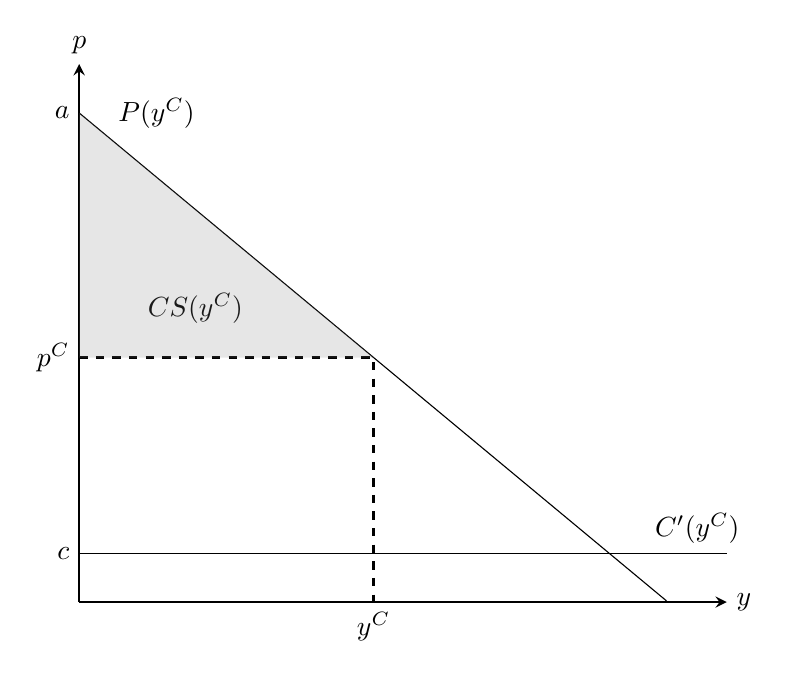
\begin{tikzpicture}
\figurename{}
\begin{axis}[
scale = 1.2,
xmin = 0, xmax = 11,
ymin = 0, ymax = 11,
axis lines = middle,
xtick = \empty , ytick = \empty,
clip = false,
axis line style = thick
]
\addplot[domain = 0:10, restrict y to domain = 0:10, samples = 400, color = black]{10-x};
\addplot[color = black, dashed, thick] coordinates {(0, 5) (5, 5) (5, 0)};
\addplot[color = black] coordinates {(0,1)(11,1)};
\node[right] at (current axis.right of origin){$y$};
\node [above] at (current axis.above origin){$p$};
\node [left] at (0, 5) {$p^C$};
\node [below] at (5, 0) {$y^C$};
\node [right] at (.5, 10) {$P(y^C)$};
\node [above] at (10.5, 1) {$C'(y^C)$};
\node [left] at (0, 10) {$a$};
\node [left] at (0,1) {$c$};
\node [right] at (1,6) {$CS(y^C)$};
\fill[gray, opacity = 0.2] (0, 10) -- (5, 5) -- (0,5);
\end{axis}
\end{tikzpicture}
\end{center}
\end{figure}
\end{document}